\documentclass[border=10pt]{standalone}
\usepackage{pgfplots}
\pgfplotsset{compat=1.18}

% Define custom colors to match the image exactly
\definecolor{barBlue}{RGB}{65, 155, 205}
\definecolor{barOrange}{RGB}{215, 105, 55}
\definecolor{barGreen}{RGB}{60, 185, 80}

\begin{document}
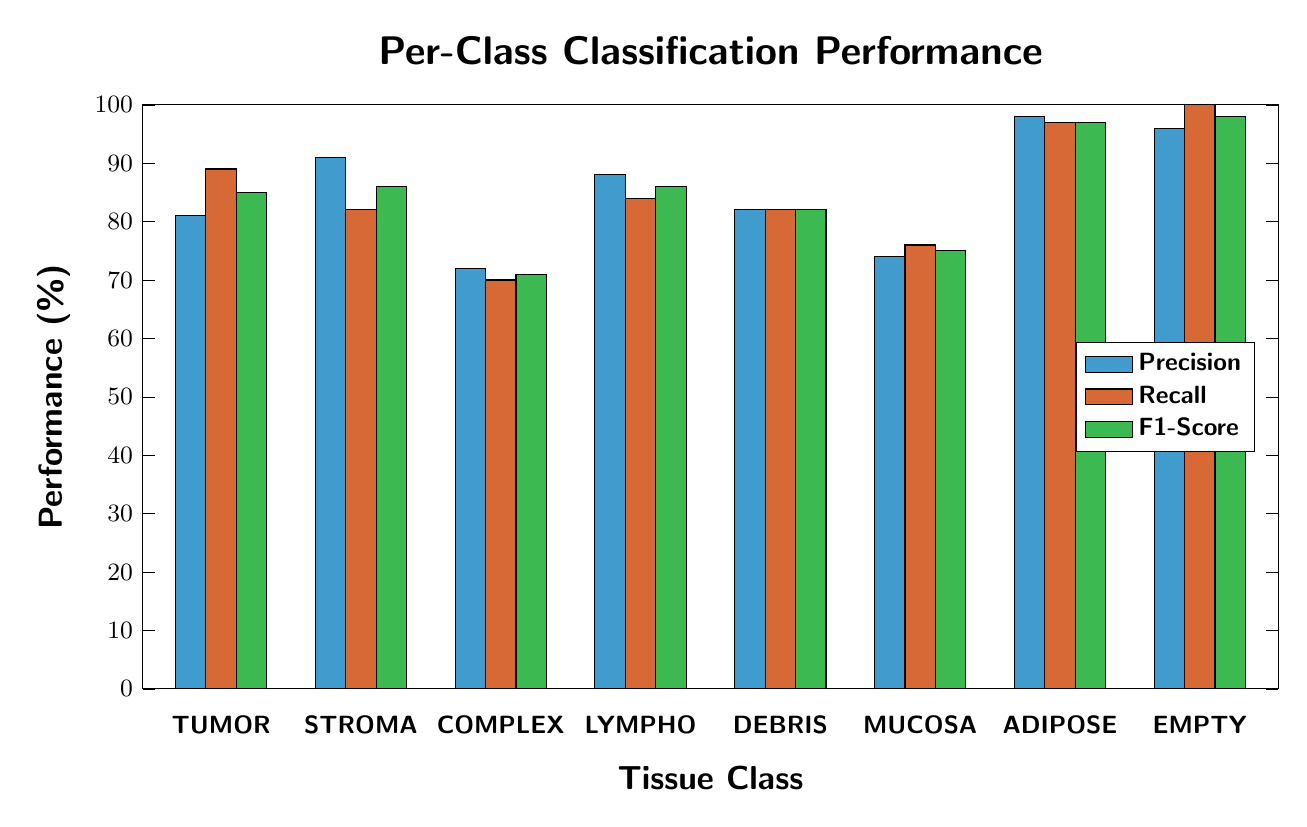
\begin{tikzpicture}
    \begin{axis}[
        ybar=0pt, % Zero spacing between bars within a group
        bar width=11pt,
        width=16cm,
        height=9cm,
        ymin=0, ymax=100,
        ytick={0,10,...,100},
        ylabel={\textbf{Performance (\%)}},
        xlabel={\textbf{Tissue Class}},
        symbolic x coords={TUMOR, STROMA, COMPLEX, LYMPHO, DEBRIS, MUCOSA, ADIPOSE, EMPTY},
        xtick=data,
        % Font and Label Styles
        xticklabel style={font=\bfseries\sffamily\small, yshift=-2pt},
        yticklabel style={font=\bfseries\sffamily\small},
        ylabel style={font=\bfseries\sffamily\large, yshift=2pt},
        xlabel style={font=\bfseries\sffamily\large, yshift=-5pt},
        title style={font=\bfseries\sffamily\Large, yshift=5pt},
        title={Per-Class Classification Performance},
        % Grid and Axis Styles
        ymajorgrids=false, % Removed horizontal grids as requested
        xmajorgrids=false,
        axis on top,
        axis line style={black},
        xtick style={draw=none},
        ytick style={black},
        enlarge x limits=0.08,
        % Legend Configuration
        legend style={
            at={(0.98,0.5)},
            anchor=east,
            font=\bfseries\sffamily\small,
            draw=black,
            fill=white,
            legend cell align=left,
            yshift=0pt
        },
        % Custom legend image to show a single colored bar
        legend image code/.code={
            \draw[#1, draw=black] (0cm,-0.1cm) rectangle (0.6cm,0.1cm);
        }
    ]

    % Precision Series (Blue)
    \addplot[fill=barBlue, draw=black] coordinates {
        (TUMOR, 81)
        (STROMA, 91)
        (COMPLEX, 72)
        (LYMPHO, 88)
        (DEBRIS, 82)
        (MUCOSA, 74)
        (ADIPOSE, 98)
        (EMPTY, 96)
    };

    % Recall Series (Orange)
    \addplot[fill=barOrange, draw=black] coordinates {
        (TUMOR, 89)
        (STROMA, 82)
        (COMPLEX, 70)
        (LYMPHO, 84)
        (DEBRIS, 82)
        (MUCOSA, 76)
        (ADIPOSE, 97)
        (EMPTY, 100)
    };

    % F1-Score Series (Green)
    \addplot[fill=barGreen, draw=black] coordinates {
        (TUMOR, 85)
        (STROMA, 86)
        (COMPLEX, 71)
        (LYMPHO, 86)
        (DEBRIS, 82)
        (MUCOSA, 75)
        (ADIPOSE, 97)
        (EMPTY, 98)
    };

    \legend{Precision, Recall, F1-Score}
    \end{axis}
\end{tikzpicture}
\end{document}